%%%%%%%%%%%%%%%%%%%%%%%%%%%%%%%%%%%%%%%%%%%%%%%%%%%%%%%%%%%%%%%%%%%%%%%%%%%%%%%%
%
% Template license:
% CC BY-NC-SA 3.0 (http://creativecommons.org/licenses/by-nc-sa/3.0/)
%
%%%%%%%%%%%%%%%%%%%%%%%%%%%%%%%%%%%%%%%%%%%%%%%%%%%%%%%%%%%%%%%%%%%%%%%%%%%%%%%%

%----------------------------------------------------------------------------------------
%	PACKAGES AND OTHER DOCUMENT CONFIGURATIONS
%----------------------------------------------------------------------------------------

\documentclass[
11pt, % The default document font size, options: 10pt, 11pt, 12pt
oneside, % Two side (alternating margins) for binding by default, uncomment to switch to one side
chapterinoneline,% Have the chapter title next to the number in one single line
spanish,
singlespacing, % Single line spacing, alternatives: onehalfspacing or doublespacing
%draft, % Uncomment to enable draft mode (no pictures, no links, overfull hboxes indicated)
%nolistspacing, % If the document is onehalfspacing or doublespacing, uncomment this to set spacing in lists to single
%liststotoc, % Uncomment to add the list of figures/tables/etc to the table of contents
%toctotoc, % Uncomment to add the main table of contents to the table of contents
parskip, % Uncomment to add space between paragraphs
headsepline, % Uncomment to get a line under the header
]{ReportPDF} % The class file specifying the document structure



%----------------------------------------------------------------------------------------
%	INFORMACIÓN DEL REPORTE
%----------------------------------------------------------------------------------------

\reporttitle{TP1: Double DQN, Dueling DQN} % El títulos de la memoria, se usa en la carátula y se puede usar el cualquier lugar del documento con el comando \ttitle

% Nombre del posgrado, se usa en la carátula y se puede usar el cualquier lugar del documento con el comando \degreename
\posgrado{Maestría en Inteligencia Artificial} 

\author{Maximiliano Torti} % Tu nombre, se usa en la carátula y se puede usar el cualquier lugar del documento con el comando \authorname

\docente{Miguel Augusto Azar}

\fechaINICIO{mayo de 2025}


\keywords{Sistemas embebidos, FIUBA} % Keywords


\begin{document}


\frontmatter % Use roman page numbering style (i, ii, iii, iv...) for the pre-content pages

\pagestyle{plain} % Default to the plain heading style until the thesis style is called for the body content

\tableofcontents % Prints the main table of contents

%----------------------------------------------------------------------------------------
%	CONTENIDO DE LA MEMORIA  - CAPÍTULOS
%----------------------------------------------------------------------------------------

\mainmatter % Begin numeric (1,2,3...) page numbering

\pagestyle{thesis} % Return the page headers back to the "thesis" style

% Incluir los capítulos como archivos separados desde la carpeta Chapters

% Chapter 1

\chapter{Desarrollo} % Main chapter title

\label{Chapter1} % For referencing the chapter elsewhere, use \ref{Chapter1} 
\label{IntroGeneral}

%----------------------------------------------------------------------------------------

% Define some commands to keep the formatting separated from the content 
\newcommand{\keyword}[1]{\textbf{#1}}
\newcommand{\tabhead}[1]{\textbf{#1}}
\newcommand{\code}[1]{\texttt{#1}}
\newcommand{\file}[1]{\texttt{\bfseries#1}}
\newcommand{\option}[1]{\texttt{\itshape#1}}
\newcommand{\grados}{$^{\circ}$}

%----------------------------------------------------------------------------------------

%\section{Introducción}

%----------------------------------------------------------------------------------------
\section{Introducción}

En el presente trabajo práctico, se desarrolla la implementación de los  algoritmos de Double-DQN y Dueling-DQN para que aprendan a jugar en forma automática al Tetris. El objetivo es poder evaluar la implementación de los algoritmo y compararlos en sus beneficios, defectos y rendimiento en un juego complejo.

Para lograrlo, se adaptó de \citep{WEBSITE:1} el ambiente de Tetris. El repositorio original ya contenía la definición de bloques, grilla, lógica de juego, puntaje y visualizaciones utilizando la libraría Pygame. Sobre esta base se agregó una clase GameUI que gestiona el flujo de visualizaciones y la interacción con los diferentes tipos de jugadores, y se agregó un método que permite obtener el estado del juego en forma codificada, necesario para entrenar modelos de aprendizaje por refuerzo basados en valor de estado. En la sección \ref{sec:entorno} se comentan mas detalles del ambiente.

Para los agentes, se adaptaron del repositorio \citep{WEBSITE:2} los algoritmos de Double-DQN y Dueling-DQN. Esta adaptación se describe con mayor detalle en la sección \ref{sec:agentes}.

Finalmente, se agrego un script principal main.py que facilita la ejecución de los casos de uso principales: entrenar los algoritmos mencionados o comenzar un nuevo juego de Tetris con interfaz visual donde el jugador es un humano o un modelo entrenado.

\section{Entorno}
\label{sec:entorno}

El juego comienza luego de definir el tipo de jugador entre las 2 posibilidades (humano o modelo de aprendizaje por refuerzo), instanciar la clase \textit{GameUI} y ejecutar el método \textit{play}. En ese instante se imprime en pantalla el tablero de la figura \ref{fig:board}. 

\begin{figure}[htbp]
	\centering
	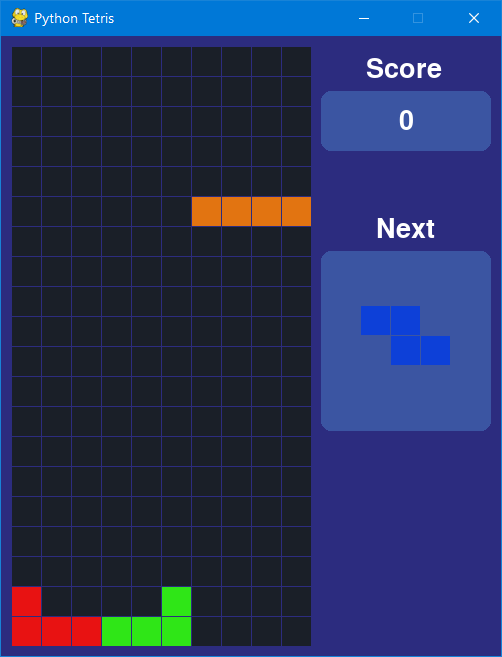
\includegraphics[width=.5\textwidth]{./Figures/tetris.png}
	\caption{Tablero de Tetris.}
	\label{fig:board}
\end{figure}

Se permiten las siguientes acciones:
\begin{itemize}
    \item Abajo: desplaza el bloque actual una posición hacia abajo.
    \item Derecha: desplaza el bloque actual una posición hacia la derecha.
    \item Izquierda: desplaza el bloque actual una posición hacia la izquierda.
    \item Rotar: rota el bloque actual 90° en sentido horario.
    \item Omitir: no realiza ninguna acción y permite que el juego continúe por si solo.
\end{itemize}

Independientemente de las acciones ejecutadas el bloque desciende una posición cada 200 ms, y cuando el bloque actual toca el ""piso"", este queda fijo y comienza a caer un nuevo bloque seleccionado aleatoriamente.

Para observar el estado del ambiente, se agregó un método que retorna una matriz de 20 filas y 10 columnas (tamaño del tablero de Tetris), donde cada elemento de la matriz es 1 si la posición respectiva en el tablero está ocupada por un bloque (ya sea el bloque actual o uno fijado) o 0 si la posición está libre. Por simplicidad no se incluyó el bloque siguiente o el puntaje actual en la observación del estado. Bajo estas condiciones, el Tetris presenta mas de \(1.6*10^{60}\) estados diferentes.

Para los puntajes, el juego base asigna 1 punto por cada ejecución de la acción abajo (de manera que el bloque descienda mas rápido), 100 puntos por completar una línea, 300 por completar 2 líneas en simultáneo y 500 por completar 3. Sobre esta lógica se agrego una quita de 5 puntos por perder el juego.

\section{Agentes}
\label{sec:agentes}

El juego admite agentes humanos o modelos de aprendizaje por refuerzo. El jugador humano puede pulsar cualquiera de las flechas para realizar la acción correspondiente (la flecha arriba ejecuta la acción rotar) cuantas veces crea conveniente. En cuanto a los modelos de aprendizaje por refuerzo, dada la enorme cantidad de estados posibles no se pueden implementar algoritmos como Monte Carlo ES o Q-Learning, ya que estos requieren crear una tabla en memoria con el seguimiento de los valores de todos los pares estado-acción. Por este motivo, se implementan los algoritmos de Doouble-DQN y Dueling-DQN que reemplazan esta tabla en memoria por una función ajustable de aproximación de los valores de estado-acción. 

El objetivo de los agentes DQN es aprender a realizar movimientos favorables en forma automática. Por simplicidad se encuentran restringidos a ejecutar un solo movimiento cada 200 ms. Es decir, en cada turno (cada 200 ms) el agente observa el estado actual del tablero, toma una de las 5 acciones posibles según su política aprendida, el ambiente se actualiza ejecutando la acción y luego moviendo el bloque actual una posición hacia abajo.

Para la arquitectura de los modelos, inicialmente se hicieron pruebas con redes densamente conectadas, pero el rendimiento conseguido fue muy pobre. En su lugar, se decidió utilizar primero capas convolucionales seguido de capas densas, como se muestra en las figuras \ref{fig:ddqn} y \ref{fig:dueling-dqn}. Estas arquitecturas recuerdan a la arquitectura básica LeNet-5. Dado que la primer capa es una capa convolucional, el estado se codificó entonces como una imagen de (20,10) pixeles con 1 solo canal.

\begin{figure}[htbp]
	\centering
	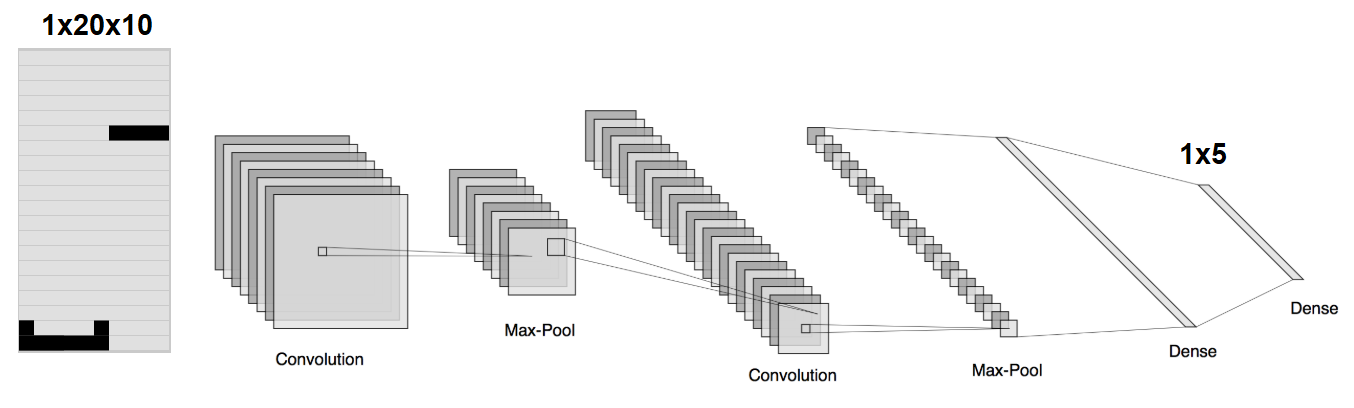
\includegraphics[width=\textwidth]{./Figures/ddqn.png}
	\caption{Arquitectura Double-DQN.}
	\label{fig:ddqn}
\end{figure}

\begin{figure}[htbp]
	\centering
	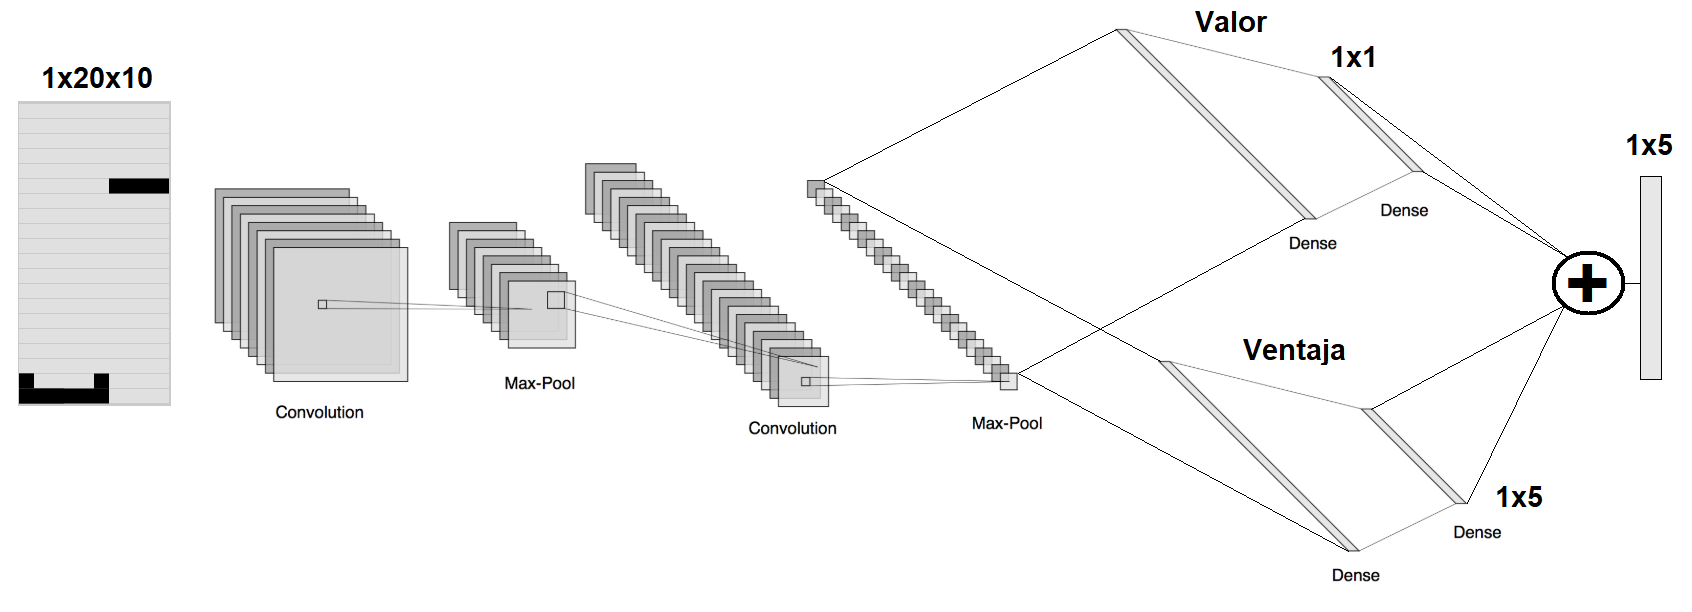
\includegraphics[width=\textwidth]{./Figures/dueling-dqn.png}
	\caption{Arquitectura Dueling-DQN.}
	\label{fig:dueling-dqn}
\end{figure}

\section{Entrenamiento}

\subsection{Double-DQN}
\label{sec:agent_double_dqn}

Para entrenar el agente de Double-DQN, se ejecutaron múltiples juegos consecutivos de Tetris con la participación del modelo en entrenamiento y sin impresión de la interfaz gráfica. Se implementó el algoritmo de \citep{ARTICLE:2} que se muestra en la figura \ref{fig:algorithm_ddqn}, con los siguientes detalles:
\begin{itemize}
    \item \(a_t\) puede tomar cualquiera de las 5 acciones posibles.
    \item \(\pi(a_t,s_t)\) sigue una política \(\epsilon\)-greedy son \(\epsilon_{inicial}=1\) y \(\epsilon_{final}=0.001\).
    \item  \(Q_\theta\) y \(Q_{\theta\prime}\) son redes DQN convolucionales que implementan la arquitectura de la figura \ref{fig:ddqn}.
    \item Las recompensas \(r_t\) son las mencionadas en la sección \ref{sec:entorno}.
    \item  \(s_t\) es una matriz de dimensiones (20,10).
    \item El replay buffer tiene un tamaño de 10.000 muestras.
    \item Se fijo un \(\gamma\) (factor de descuento) de \(0.9\). 
    \item Para el entrenamiento de gradiente descendiente se utilizó un batch de 64 muestras y un lr de \(0.001\).
    \item La red objetivo se actualizó cada 100 actualizaciones de gradiente.
    \item El entrenamiento se repitió durante 1.000 episodios, demorando aproximadamente 1 hora.
\end{itemize} 

\begin{figure}[htbp]
	\centering
	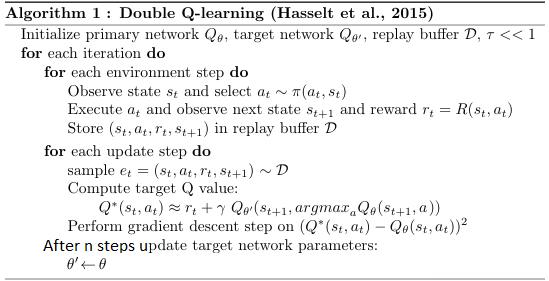
\includegraphics[width=0.8\textwidth]{./Figures/algorithm_ddqn.png}
	\caption{Algoritmo de Double-DQN.}
	\label{fig:algorithm_ddqn}
\end{figure}

\subsection{Dueling DQN}

Para entrenar el agente de Dueling-DQN, se replicó el mismo proceso que en la sección \ref{sec:agent_double_dqn}, con el mismo algoritmo de figura \ref{fig:algorithm_ddqn}, difiriendo solamente en la implementación de \(Q_\theta\) y \(Q_{\theta\prime}\) que en este caso son redes convolucionales que implementan la arquitectura de la figura \ref{fig:dueling-dqn} y calculan por separado el valor general de un estado y las ventajas de cada acción en ese estado.

\section{Resultados}

\subsection{Double-DQN}

Luego de entrenar el agente Double-DQN por 1.000 episodios se obtuvo la curva de recompensa de la figura \ref{fig:ddqn_rewards}.

Se observa que la media móvil de la recompensa aumenta lentamente con el paso de los episodios desde un valor de 30 hasta aproximadamente 100, lo que indica que el modelo está entrenándose. No obstante, dado el puntaje, es de suponer que la política que se está aprendiendo no es la de completar líneas, ya que cada línea simple completada otorga 100 puntos. Si observamos la evolución de la recompensa sin filtrar, si notamos que cada ciertos episodios obtenemos recompensas mayores a 200 e incluso 300, por lo que en ciertos casos el agente logra completar líneas.

\clearpage

\begin{figure}[hbt!]
	\centering
	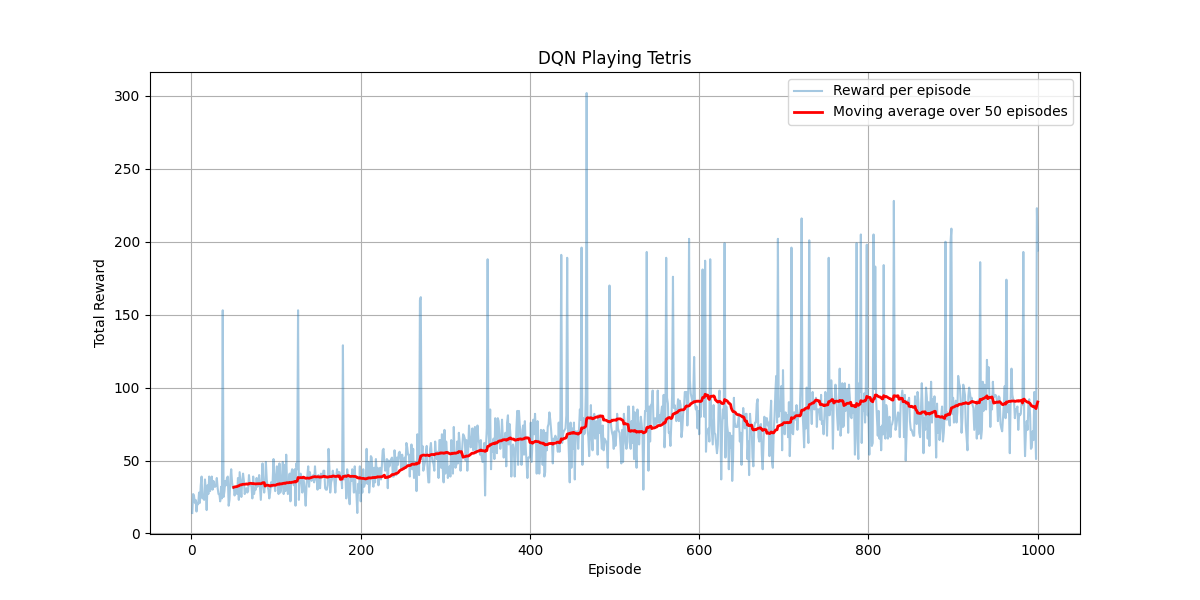
\includegraphics[width=\textwidth]{./Figures/ddqn_rewards.png}
	\caption{Recompensa por episodio para algoritmo de Double-DQN, suavizado con una media móvil de 50 episodios.}
	\label{fig:ddqn_rewards}
\end{figure}

Al ejecutar el juego con el modelo entrenado como jugador, se observa que intenta completar lo máximo posible la grilla pero con una política muy básica. Solo distribuye los bloques a lo ancho del tablero (para extender perder el juego) con pocas o nulas rotaciones, e intenta bajar los bloques lo más rápido posible con la acción abajo para obtener los puntos de recompensa que esto otorga, como muestra la figura \ref{fig:ddqn_playing}. Ocasionalmente, la política anterior completa una línea, como en la figura \ref{fig:ddqn_playing_line}, pero solo por coincidencia, el modelo no busca activamente completar lineas. En la sección \ref{sec:conclusions} se detallaran las razones de este resultado poco satisfactorio.

\begin{figure}[hbt!]
	\centering
	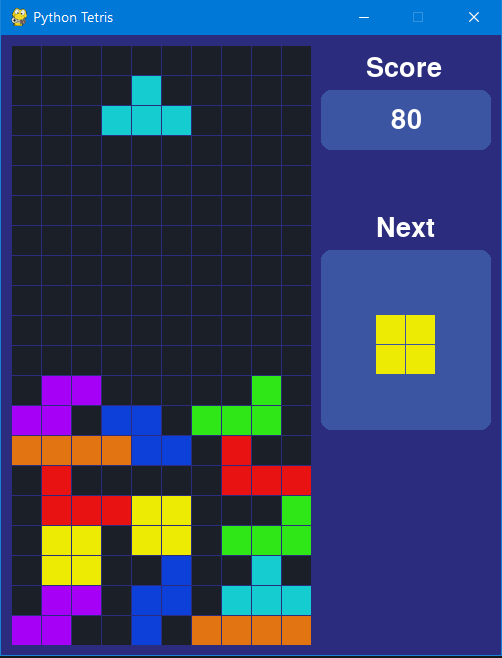
\includegraphics[width=0.5\textwidth]{./Figures/ddqn_playing.png}
	\caption{Agente Double-DQN distribuyendo bloques a lo ancho del tablero.}
	\label{fig:ddqn_playing}
\end{figure}

\begin{figure}[htbp]
	\centering
	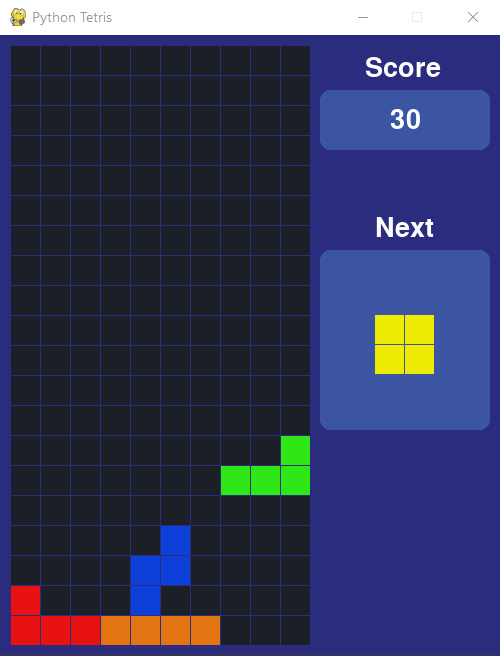
\includegraphics[width=0.5\textwidth]{./Figures/ddqn_playing_line.png}
	\caption{Agente Double-DQN completando una línea.}
	\label{fig:ddqn_playing_line}
\end{figure}

\subsection{Dueling-DQN}

Al entrenar el agente Dueling-DQN por 1.000 episodios, se obtuvo la curva de recompensa de la figura \ref{fig:dueling_dqn_rewards}.

\begin{figure}[htbp]
	\centering
	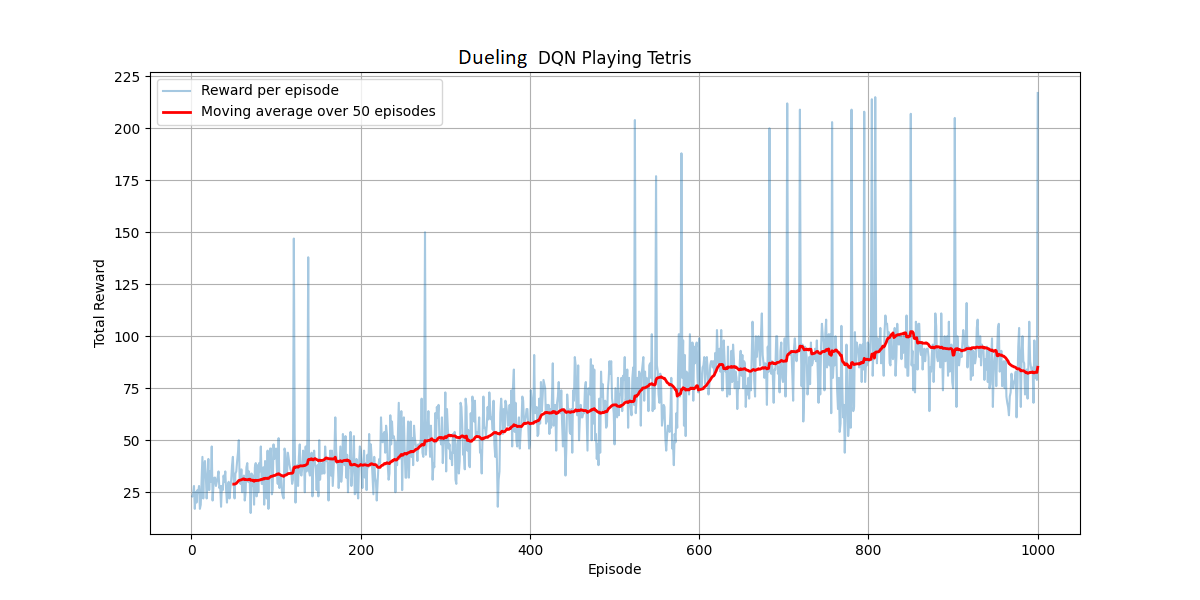
\includegraphics[width=\textwidth]{./Figures/dueling_dqn_rewards.png}
	\caption{Recompensa por episodio para algoritmo de Dueling-DQN, suavizado con una media móvil de 50 episodios.}
	\label{fig:dueling_dqn_rewards}
\end{figure}

La curva muestra leves mejoras, aunque poco apreciables. Al ejecutar el juego con el modelo entrenado como jugador, se observa que este modelo realiza una mejor distribución de los bloques a lo ancho del tablero, como se muestra en figura \ref{fig:dueling_dqn_playing}, pero tiene las mismas limitaciones que el algoritmo anterior.

\clearpage

\begin{figure}[htbp]
	\centering
	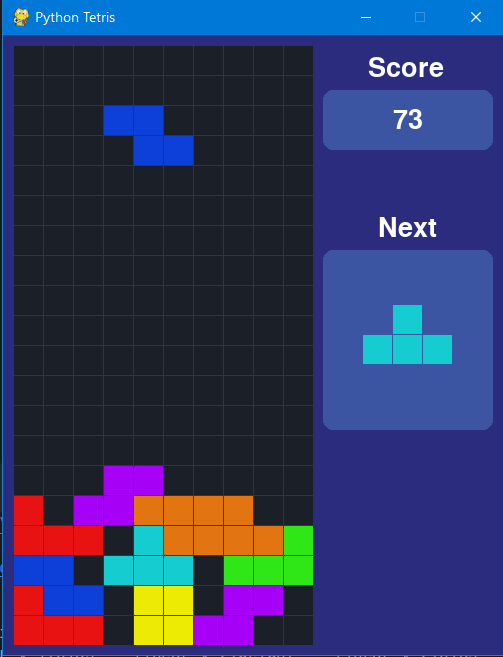
\includegraphics[width=0.5\textwidth]{./Figures/dueling_dqn_playing.png}
	\caption{Agente Dueling-DQN distribuyendo bloques a lo ancho del tablero.}
	\label{fig:dueling_dqn_playing}
\end{figure}

A fin de verificar que el rendimiento no esté siendo limitado por la cantidad de episodios, se continuó el entrenamiento de este caso durante 10.000 episodios más, demorando aproximadamente 10 horas. La curva de recompensa obtenida se muestra en la figura \ref{fig:dueling_dqn_rewards_10k}.

\begin{figure}[hbt!]
	\centering
	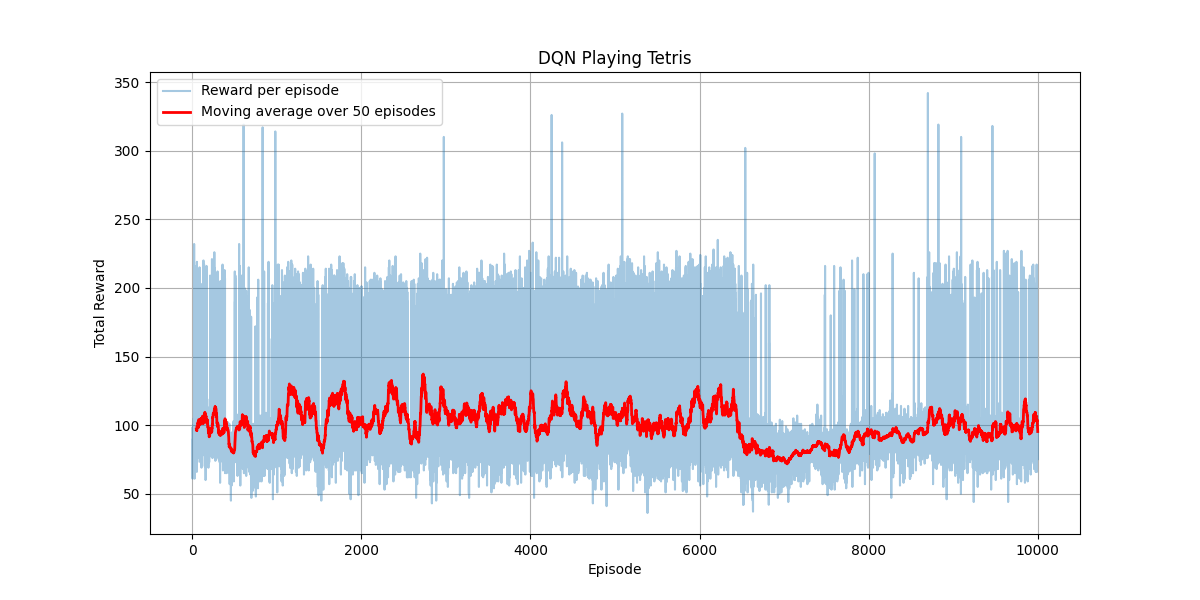
\includegraphics[width=\textwidth]{./Figures/dueling_dqn_rewards_10k.png}
	\caption{Recompensa por episodio para algoritmo de Dueling-DQN luego de 10.000 episodios, suavizado con una media móvil de 50 episodios.}
	\label{fig:dueling_dqn_rewards_10k}
\end{figure}

Ahora, en la mayoría de episodios el modelo completa una o dos líneas, pero nuevamente la media no supera la barrera de los 150 puntos. Es decir, el modelo sigue aprendiendo simplemente a distribuir bloques y el aumento de la cantidad de episodios no mejora sustancialmente los resultados obtenidos.

\section{Conclusiones}
\label{sec:conclusions}

Ambos algoritmos mostraron resultados poco satisfactorios, aprendiendo solamente una política básica de distribuir bloques y extender el juego lo máximo posible pero no de completar líneas. 

Comparando, Dueling-DQN obtuvo resultados levemente mejores gracias a que separa el cálculo del valor general para el estado actual y de la ventaja que se conseguiría ejecutando cada acción, lo cual es beneficioso en un caso como el del juego del Tetris donde todas las acciones tienen aproximadamente la misma recompensa (valor general) y algunas acciones representan un pequeño valor agregado (ventaja).

Al analizar en detalle la limitación de los algoritmos para este caso, se concluyó lo siguiente:
\begin{itemize}
    \item Ambos algoritmos se basan en \(TD(0)\), lo que provoca que sean extremadamente codiciosos y busquen la recompensa inmediata. Esto es contraproducente en un juego como el Tetris donde la recompensa real (completar líneas) se obtiene luego de más de 50 pasos futuros correctos. 
    \item Estas variantes de DQN basadas en \(TD(0)\) realizan estimaciones de \(Q(t)\) y \(Q(t+1)\) que pueden presentar un gran error de bias en entornos complejos. Por lo tanto, es de esperar que el incremento del valor de estado obtenido por completar una línea luego de 50 pasos futuros no se vea reflejado correctamente en las estimaciones de valor del estado actual o inmediato próximo que realizan la redes neuronales.
    \item El Tetris requiere ejecutar correctamente múltiples pasos consecutivos para llegar a estados favorables. Es muy poco probable que la política \(\epsilon\)-greedy logre una buena exploración del espacio de estados y acciones posibles. Entonces, el modelo tendrá muy pocas instancias de movimientos correctos para ajustar su política, y muchas instancias de movimientos que no aportan valor en su entrenamiento.
\end{itemize}
Para poder resolver estas problemáticas se puede o bien usar otro algoritmo que tenga menor error de bias en la estimación de los valores de estado (como Actor-Critic), o modificar los algoritmos utilizados de DQN. Como ejemplo, \citep{ARTICLE:1} plantea utilizar una variante de DQN con los siguientes cambios:
\begin{itemize}
    \item Agregar pre-entrenamiento con episodios jugados por humanos (llamado demostración), que poseen mayor concentración de muestras con pares estado-acción favorables.
    \item Realizar un muestreo ponderado del replay buffer al obtener los batch de entrenamiento de la red neuronal, priorizando los pasos de episodios que hayan conseguido altos puntajes. 
    \item Modificar la función de pérdida de la red neuronal:
    
    \(J(Q) = J_{DQ}(Q) + \lambda_1 J_n(Q) + \lambda_2 J_E(Q) + \lambda_3 J_{L2}(Q) \)
    
    Donde \(J_{DQ}(Q)\) es el error clásico \(TD(0)\), \(J_n(Q)\) es el error TD(n) qu permite disminuir el error de bias mencionado, \(J_E(Q)\) está solo presente en el pre-entrenamiento y es un término de error cross-entropy que fuerza a la red a seguir los pasos que siguió el humano, y  \(J_{L2}(Q)\) es un término de regularización L2 para evitar el overfitting.
\end{itemize}
Lamentablemente la implementación de ambas soluciones escapan del alcance de este proyecto y se enuncian como trabajo futuro.

\section{Trabajo futuro}

Como trabajo futuro se plantea implementar y comparar las soluciones a las limitaciones encontradas en los algoritmos de Double-DQN y Dueling-DQN en el juego de Tetris, mencionadas en la sección \ref{sec:conclusions}:
\begin{enumerate}
    \item Implementar un algoritmo que posea menor error de bias en la estimación del valor de estado como, por ejemplo, Actor-Critic.
    \item Implementar las técnicas de demostración humana, muestreo ponderado sobre el replay buffer y función de pérdida modificada sobre Dueling-DQN.
\end{enumerate}
\include{Chapters/Chapter2} 
\include{Chapters/Chapter3}
\include{Chapters/Chapter4} 
\include{Chapters/Chapter5} 

%----------------------------------------------------------------------------------------
%	CONTENIDO DE LA MEMORIA  - APÉNDICES
%----------------------------------------------------------------------------------------

\appendix % indicativo para indicarle a LaTeX los siguientes "capítulos" son apéndices

% Incluir los apéndices de la memoria como archivos separadas desde la carpeta Appendices
% Descomentar las líneas a medida que se escriben los apéndices

% Appendix A

\chapter{Script principal} % Main appendix title

\label{Script principal}

El script principal del proyecto contiene un procesador de líneas de comando que facilita la ejecución de los diferentes casos de uso. Los usos básicos del procesador se detallan a continuación:

\begin{itemize}
    \item Mostrar la ayuda.
\end{itemize}
\begin{verbatim}
$ python -m src.main --help
\end{verbatim}

\begin{itemize}
    \item Jugar al Tetris con el teclado.
\end{itemize}
\begin{verbatim}
$ python -m src.main play --human
\end{verbatim}

\begin{itemize}
    \item Entrenar un nuevo agente de Double-DQN.
\end{itemize}
\begin{verbatim}
$ python -m src.main train --model=ddqn
\end{verbatim}

\begin{itemize}
    \item Entrenar un nuevo agente de Dueling-DQN.
\end{itemize}
\begin{verbatim}
$ python -m src.main train --model=dueling-dqn
\end{verbatim}

\begin{itemize}
    \item Ejecutar el juego Tetris con un agente Double-DQN entrenado.
\end{itemize}
\begin{verbatim}
$ python -m src.main play \
    --model-file="./resources/ddqn/model_ddqn.pkl" --model=ddqn
\end{verbatim}

\begin{itemize}
    \item Ejecutar el juego Tetris con un agente Dueling-DQN entrenado.
\end{itemize}
\begin{verbatim}
$ python -m src.main play \
    --model-file="./resources/dueling_dqn/model_dueling_dqn.pkl" \
    --model=dueling-dqn
\end{verbatim}

\begin{figure}[htbp]
	\centering
	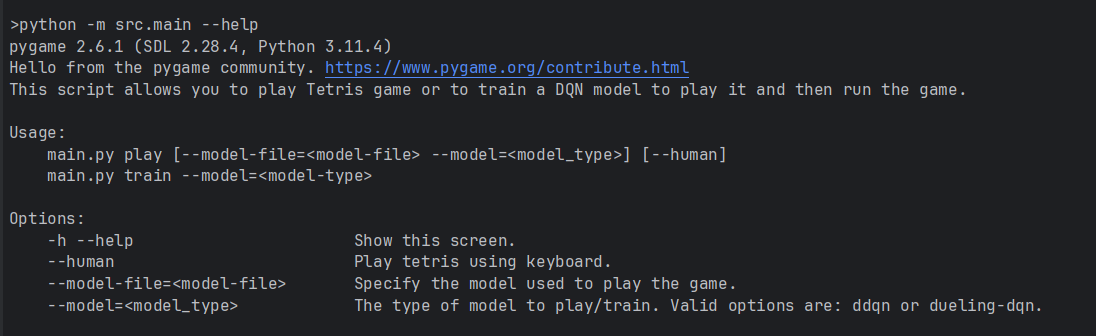
\includegraphics[width=\textwidth]{./Figures/command.png}
	\caption{Uso del script principal por línea de comando.}
	\label{fig:command}
\end{figure}
% Appendix B

\chapter{Calidad de código} % Main appendix title

\label{Cobertura y calidad de código}

Para mantener una buena calidad de código, el repositorio cuenta con documentación extensiva y un archivo README.md donde se detalla el uso del proyecto. Adicionalmente se ejecutaron análisis estáticos de calidad de código mediante la herramienta SonarLint y se resolvieron las malas prácticas y los problemas de seguridad encontrados.

\begin{figure}[htbp]
	\centering
	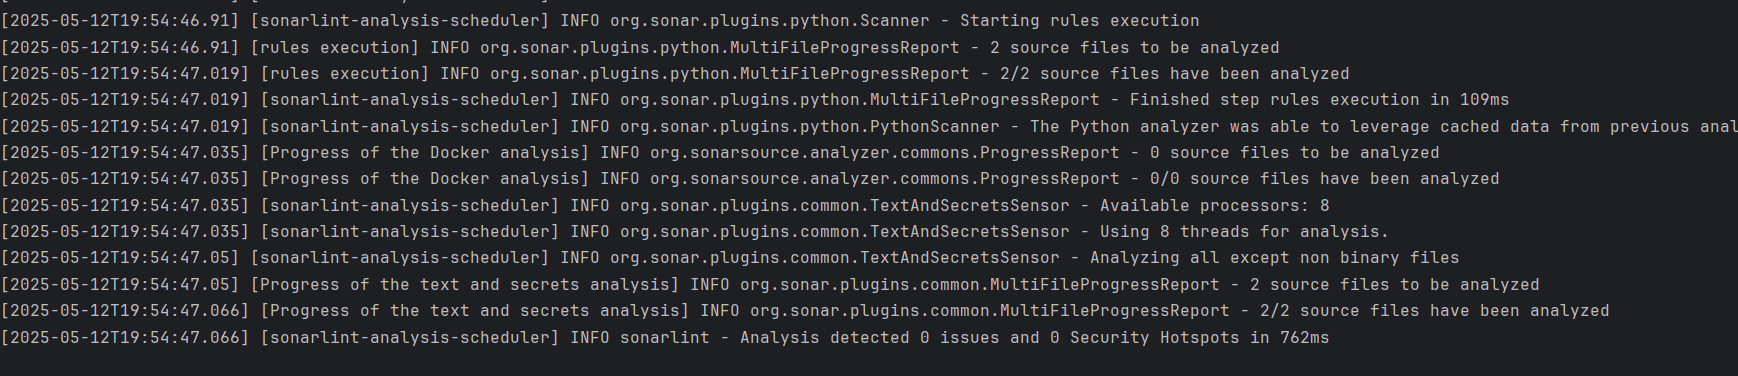
\includegraphics[width=\textwidth]{./Figures/sonar.png}
	\caption{Análisis estático de código.}
	\label{fig:sonar}
\end{figure}


% Appendix C

\chapter{Repositorio} % Main appendix title

\label{Repositorio}

El repositorio con el código fuente y archivos adicionales de utilidad se encuentra disponible en el siguiente link:

\url{https://github.com/maxit1992/MIA_RL2/tree/master/tp1}



%----------------------------------------------------------------------------------------
%	BIBLIOGRAPHY
%----------------------------------------------------------------------------------------

\Urlmuskip=0mu plus 1mu\relax
\raggedright
\printbibliography[heading=bibintoc]

%----------------------------------------------------------------------------------------

\end{document}  
